% LLNCS class package used for SMU Data Science Review Journal
\documentclass{llncs}

% Packages to be used in the document
\usepackage{graphicx} % display figures sample figures - EPS format (preferred), PDF/JPEG also acceptable
\usepackage{booktabs} % Better horizontal rules in tables
\usepackage{multirow} % Better combined rows in tables
\usepackage{xcolor} % Change font color for editing purposes
\usepackage{hyperref} % Footnote references
\usepackage{mathtools}
\usepackage{makecell}
\usepackage{url}
%\graphicspath{ {./images/} }

% change intro to have Background super section with Tutorial to explain SVM/KMeans/AVC, and Related works with lit review -- Michael 

%Citations should all be APA compliant





% Paper Title
\title{\textbf{Fall Detection: Threshold Analysis of Wrist-Worn Motion Sensor Signals}}

% Complete List of Authors with Affiliations
\author{Joseph Caguioa\inst{1}\and Andy Nguyen\inst{1}\and  Michael J. Wolfe\inst{1}\and Jacquelyn Cheun\inst{1}} %Capstone Advisor: Jacquelyn Cheun

\institute{Master of Science in Data Science, Southern Methodist University, Dallas TX 75275 USA
	      \email{\{jcaguioa, andynguyen, mwolfe, \& jcheun\}@smu.edu} 
	      % \and Add further credentials/companies for yourselves @Michael/Joseph
	      }	  
% Begin Document 
\begin{document}
% Typeset the title & authors of paper
\maketitle
% Reset footnote counter
%\setcounter{footnote}{0}

% Abstract Typeset
% REWRITE ABSTRACT
\begin{abstract}
In this paper, we present a detection algorithm that accurately differentiates the event of a person falling from normal Activities of Daily Living (ADL). Our algorithm processes signals recorded from accelerometers and gyroscopes built into wearable activity monitoring devices such as smart watches that are worn on an individual's wrist. Existing algorithms are accurate but imprecise, and rely too much on inconveniently-placed sensors. We propose a pipeline that improves precision without sacrificing accuracy and ease of use. We present the use of a combination of threshold-based and machine learning-based approaches to develop a refined fall-detection algorithm that builds upon previous research. Using various pre-processing techniques such as magnitude and acceleration change vectors, our model labels the varied activities into falls and ADLs using k-means clustering. Finally, we test the accuracy of these labels in a Support Vector Machine (SVM) binary classifier. Our hope, given the potential danger of injury resulting from a fall, is to create an accurate and precise fall detection algorithm that could be the precursor to an autonomous emergency alert system. 
%  Need to include - two to three sentences are used to state how the problem was solved. A single statement of the main result (singular) is then followed by a single statement of the main conclusion (singular).
\keywords{fall detection \and threshold analysis \and Activities of Daily Living (ADL) \and signal processing \and Acceleration Vector Change (AVC) \and Angular Velocity Vector Change (WVC) \and K-Means Clustering \and Support Vector Machines (SVM) \and wrist-worn triaxial motion sensors \and }
\end{abstract}

% We most likely need to include a Related Works subsection to discuss previous ideas we might take when building our own algorithm.
% add Background - related

% Note that paragraphs are created by placing a blank line before the 
% paragraph within the .tex file just as a blank line exists before the
% beginning of this comment. That blank line tells LaTeX to treat the 
% following text as a new paragraph.  No other commands are needed.


% Sections are denoted by the use of the \section{Section Name} 
% command -- where "Section Name" is the name you give to the Section.
\section{Introduction}

The elderly are most prone to the dangers of falling that may significantly impair their daily lifestyle. Non-fatal falls often result in severe physical injuries such as broken bones, internal tissue damage, and head trauma. However, these falls for the elderly population can also result in persisting psychological fears due to post-traumatic stress and are at the highest risk of a reoccurring incident. The World Health Organization (WHO) report that fatality rates from falls are consistent with risk factors of advanced age and other associated predispositions such as: 1) reduced activity from physical depreciation; 2) chronic underlying medical conditions, including arthritis, neurological diseases, and cardiac diseases; 3) side effects from increased use of prescription medications, that can have compounding effects on the central nervous system;  4) hazardous environments; and 5) substance abuse.\footnote{\url{https://www.who.int/news-room/fact-sheets/detail/falls}} Fall prevention has been investigated as a proposed solution, taking preemptive measures to reduce the number of falls, but accidental falls can not always be averted.  In 2016, approximately 30,000 adults aged 65 years and older died as the result of fatal falls in the United States, the leading cause of injury-related fatalities within this age range.\cite{burns2018deaths} The adjusted-age death rates for this senior population have increased by 31\% from 2007 to 2016, with an estimated 43,000 deaths due to fatal falls in 2030 if these current rates remain stable.\cite{burns2018deaths} Autonomous fall detection systems have since been developed with the intention of quickly identifying senior falls to provide immediate interventions if necessary in an effort to combat these increasing mortality rates.

	The critical danger of a fall is being in a ``long-lie'' condition, in which the person remains on the ground for an extended period unable to help themselves up after a fall.\cite{bagala2012evaluation} This may result in severe loss of self-confidence in fortunate situations of non-bodily harm, but in more grave cases potentially result in life-threatening complications such as a Traumatic Brain Injury (TBI) induced by head trauma from the fall. The Centers for Disease Control and Prevention (CDC) reported in 2014 that falls were the leading cause for TBI, accounting for roughly half (48\%) of TBI-related emergency department visits.\footnote{\url{https://www.cdc.gov/traumaticbraininjury/get_the_facts.html}} Patients can suffer extended periods of unconsciousness in a critical ``long-lie'' condition in urgent cases of traumatic brain injuries, unable to help themselves or request for immediate assistance. 
	
	From a survey obtained on 125 subjects ages 65 and older, half of those who suffered a ``long-lie'' state for over an hour died within six months following the first reported fall.\cite{wild1981dangerous} Fall detection systems help address the concerns of ``long-lie'' falls by identifying when falls occur and dispatching immediate assistance in order to minimize the period of time individuals remain helpless. The first fall detection system proposed was a personal alarm system (PAS), in which a user-activated device could be worn as a wristband or necklace, but required the user to be conscious after a fall has occurred to press the button and alert an emergency help desk operator.\cite{de2015towards} The issue with these initial systems is that they did not consider severe cases in which individuals lose consciousness and are unable to activate the alarm signal for assistance. Since then, novel autonomous fall detection systems have been introduced that do not require a user-activated alert signal; they can be categorized into: camera-based systems, ambient environment sensor-based systems, and wearable sensor-based systems. 	
	
	Advancements in wearable sensors and system over the past decade has generated interest in using wearable technology to support clinical assessments of patients. Potential applications from these developments have shown promise in early diagnosis of cardiac diseases such as congestive heart failure, prevention of chronic conditions such as diabetes, improvement in clinical management of neuro-degenerative conditions such as Parkinson's disease, and the ability to promptly respond to emergency situations such as cardiac arrest or TBI.\cite{bonato2010wearable} Currently, wearable technologies have been commercialized on the market as smartwatch accessories that include features for activity monitoring, physical fitness tracking, and global positioning systems (GPS). A 2019 survey conducted by the Pew Research Center reports that one in every five Americans (21\%) are estimated to wear a smartwatch or fitness tracker regularly, producing massive amounts of data that can be used for healthcare research.\footnote{\url{https://www.pewresearch.org/fact-tank/2020/01/09/about-one-in-five-americans-use-a-smart-watch-or-fitness-tracker/}} Considering how wide-spread the use of these devices are currently, we believe autonomous fall detection research primarily focused on sensor placements on the wrist will have the most potential as a universal real-world application to address concerns regarding the mortality rates from falls.
	
	Unfortunately, prior research testing fall detection reliability have found that false positive rates are high when using a single wrist sensor.\cite{gjoreski2016accurately} Generally, torso, waist and head based sensors have proven to be more effective in detecting falls, but in this study, wrist-based sensors were still able to detect faster falls with some accuracy. While waist placement has the benefit of aligning to the human anatomy's center of gravity, sensor placement at the head has produced superior impact detection sensitivity. Triaxial accelerometer data from both sites produced efficient fall detection algorithms with a sensitivity around 97\% and specificity of 100\%, even with simple threshold-based algorithms.\cite{kangas2008comparison} Although evidence suggests that sensors placed at the head and waist yielded the most accurate predictions, we only investigate how wrist sensor data can be used to train an autonomous fall-detection algorithm for its potential application in smartwatch accessories.
	
	%Prior research on fall-detection algorithms using triaxial accelerometers has shown that applying identified fall events from a simple threshold model to a Hidden Markov Model produced the most accurate results and was a more efficient algorithm that required less computational resources.\cite{lim2014fall} We will analyze how competing algorithms perform when combining a simple threshold-based model to detect potential falls with different machine learning-based models. We are specifically interested in observing how Linear Discriminant Analysis (LDA), Support Vector Machines (SVM), Naïve Bayesian (NB), Decision Trees (DT), and Random Forests (RF) compare on a binary classification task that differentiates a fall from an ADL. We will compare these competing models based on their classification accuracy, specificity, sensitivity, and precision. In order to accurately discriminate ADLs, we will consider clustering techniques to analyze patterns in accelerometer and gyroscope data from wrist sensors to understand how different classes of daily living activities are identified in our algorithm. The goal of our research is to present an optimized fall-detection algorithm based on a simple threshold and machine learning models that can be implemented into wearable wrist devices such as smartwatches. 
	
	%We propose a novel autonomous fall-detection system using algorithms trained on data extracted from wireless accelerometer and gyroscope wrist sensors as a potential solution to address these concerns. When our algorithm detects a fall and the user is unable to confirm consciousness through the wrist device, it could trigger an alert to dispatch local paramedics to the device's exact GPS location for an emergency evaluation and immediate medical intervention. %The algorithm is tasked with a binary classification that will discriminate actual falls from typical activities of daily living: bathing, ambulatory, transferring, toileting, eating, and dressing.

	%Cluster the data by ADL to find patterns in accelerometer and gyroscope data
	%PCA on accelerometer and gyroscope data to reduce data dimensionality. The data will have data for those features in 3 dimensions (x, y, z) and make intuitive sense to be reduced into just one accelerometer and one gyroscope feature.
% Results Summary
% Conclusion Summary

% May need to restructure this final paragraph in Introduction
	%Intro -> Background (Related Works) -> Methods (Data) -> Results (Model comparsions) -> Discussion (Ethics) -> Conclusions
	The remainder of this paper is organized into the following sections. Section two will discuss related studies that have guided our work and analyzed the efficacy of previous implementations of autonomous fall-detection systems. Section three will discuss methodologies: how the data was collected along with its structures and processing methods, as well as a high-level overview of the machine learning concepts applied to develop our solution. Section four will present the results of our findings accompanied with tables and figures to summarize the analysis. Section five will wrap up our analysis with ethical considerations and potential implications of handling personal health data recorded from wearable wrist devices. Section six will summarize our main conclusions and potential ideas to refine our proposed solution. 
% Ethics
	% Testing elderly patients: the experiments and activity are more taxing for them compared to relatively younger individuals. Could be a possible explanation for why datasets do not heavily test on that specific age group despite that being the targeted population for applicable use.
	% Privacy concerns with sharing constant GPS location
	% False positives can amount to increased fall-related costs (i.e. non-essential dispatch of paramedics)

% The average life expectancy for U.S. citizens estimated to be 78.6 years of age. \footnote{\url{https://www.cdc.gov/nchs/fastats/life-expectancy.htm}} 
%\section{Background}
Fall detection is a rich field with considerable depth and breadth. Much work has been done on all levels, from algorithms to detect falls from certain positions or heights to simply studying and defining movement in general.
\section{Related Works}
  One of the most prominent studies for our purposes is the Burns study on fall-related deaths in the elderly.\cite{burns2018deaths} This is the primary impetus for our project: fall-related deaths are common and preventable with timely intervention.
    
    In \cite{noury2007principles}, fall scenarios are categorized for evaluation purposes: namely forward, backward, and lateral. Fall-like scenarios such as syncope, where a fainted individual slips down a wall into a sitting position, are also mentioned. Such categorizations are later used in many studies for fall events.
     
    Methods that use accelerometers to detect a fall typically analyze data about a person's acceleration before, during, and after the event. Terminology varies between studies, but most describe the segmentation in the following chronological order: a normal ADL period succeeded by a sudden spike in acceleration within a short time window, followed by a sudden deceleration on impact, followed by an extended period of no acceleration if the person is in a ``long-lie'' state. Events with slower falls or multiple impacts may have slightly different profiles of acceleration over time.\cite{kangas2009sensitivity}
    
    Prior fall detection research suggests processing raw triaxial sensor measurements into magnitude signal vectors to reduce dimensionality. From the acceleration magnitude vector, an Acceleration Vector Change (AVC) feature can be extracted to capture motion intensity. Stronger motions will result in sudden, drastic changes in the acceleration signal and produce greater AVC values.\cite{gjoreski2016accurately} Gjoreski's various studies compared the effectiveness of different fall detection models trained using this feature at four positional sensors (wrist, head, waist, and thigh), finding a Random Forest model to perform the best overall with an accuracy of 80\%. However, his research indicated that a Support Vector Machine (SVM) classifier was more accurate on just wrist sensor data. 
 
    %In our literature review, we discovered that many fall detection studies had implemented similar pre-processing of their data. By combining accelerometer data with sensor metrics, researchers created Acceleration Vector Changes. This is a vector of acceleration changes by sensor, indicating the subject's motion in a given period of time. %This can be tested in a variety of methods, ranging from a simple threshold analysis to training a classification algorithm. For example, their early work compared different classifiers and their effectiveness in detecting falls. Using four positional sensors (wrist, head, waist, and thigh), they calculated AVC's and trained Bayesian, Random Forest, and SVM classifiers, among several others. Overall, they found Random Forest to be the most accurate at roughly 80 percent. However, when looking at just the left wrist sensor, SVM was more accurate. Since we are testing only wrist-based sensors due to their practicality, this would indicate a combination of pre-processing AVCs then using SVM to classify falls could be a winning ensemble.\cite{gjoreski2016accurately}
 
    In a different study using similar methods, Hussain et al. used a low-pass Butterworth filter to pre-process their data. A low-pass Butterworth filter is a common technique in signal processing, used to filter out noise components in a signal system. In our case, the noise would be gravity itself. If we represented our problem of discerning acceleration in an activity, ADL or otherwise, from gravity, we would represent it thusly:
    
    %\begin{figure}
    %\centering
    %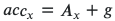
\includegraphics[width=2cm, height=.5cm]{images/acc_formula.png}
    %\end{figure}
    
\begin{equation*}
	acc_{x} = A_{x} + g
\end{equation*}
    
Where acc is the overall acceleration, A represents the activity-based acceleration and g represents gravity. A low-pass Butterworth filter would decompose this equation into A and g, and allow the researcher to determine if A represents a fall or an ADL. This enables researchers to a subject's effect on its acceleration in space. After pre-processing, the researchers compared various classifiers and their efficacy in predicting falls and found SVM to be the most accurate at 99.98\%, further verifying the viability of SVM classifiers in detecting falls.\cite{hussainelderly2019}
    
    %Aside from data processing techniques, another widely explored field in fall detection is the number, placement, and type of sensor used to detect falls. As mentioned above, Gjoreski's study uses sensors in the waist, thigh, wrist, and head. Each sensor is found to have different levels of accuracy depending on which model was uses. For example, Random Forest on the head-mounted sensor was the most accurate of all models and sensors. However, using SVM the left-wrist-based sensor produced a fairly accurate model.\cite{gjoreski2016accurately} For our purposes we will focus on a sensor based on the left wrist. From a practicality standpoint this is the best approach. Popular products today equipped with fall detection technology are generally smart watches, worn on the left wrist. Given that our algorithm is likely to see broader adoption if geared towards smart watches, we will focus on methods that are based on these types of sensors.

%\subsection{Tutorial}

%The three primary techniques leveraged in our model are Acceleration Vector Changes, K-Means Clustering, and Support Vector Machines. Each of these techniques, in ensemble, form the final state of our fall classification pipeline. This represents a synthesis of multiple previous efforts discussed in our Related Works, along with our own analysis of the data.

%add more detail to each

%Acceleration Vector Changes are a signal processing method of calculating the per-trial acceleration vector.

%A high level diagram on machine learning could be really nice here, especially explaining the differences between subtypes, starting at supervised and unsupervised and drilling down

%K-means clustering is an unsupervised learning technique by which unlabelled input vectors are assigned squared Euclidean distances from k-centroids. Typically, the user defines the number of expected clusters in order to create labels for the data. K-means is rooted in signal processing and data mining, thus it is a strong choice for the problem at hand.

%Specifically, we are using k-means to create labels for our dataset. Since we already know we want to define the input vectors into falls and ADLs from the various activities, k-means will group and label these vectors accordingly.

%Support Vector Machines are a supervised machine learning technique wherein, given a 2D feature space, a hyperplane (also known as a decision boundary), is defined which separates one class from another. It requires labelled data to define these classes, and relies on kernels (mathematical functions to elevate the feature space) to define the hyperplane.

%We use a SVM to classify centroid distances generated from k-means to predict falls vs ADLs. We will need to test a variety of kernels, since the k-means feature space may or may not be linear, quadratic, or possibly separable in a 3D feature space. We will use accuracy and precision as competitive measures to determine which kernel is best in our final model.
    
\section{Materials and Methods}
Our study uses a subset of the UP-Fall Detection dataset to analyze acceleration and angular velocity signals measured on wrist-worn sensors to simulate smartwatch placement.
\subsection{Data}

The UP-Fall Detection dataset is used to analyze and compare the different methods for detecting falls through wrist sensors. The complete dataset is a collection of information from five wearable sensors, six infrared sensors, two cameras, and an electroencephalograph headset. Mart{\'\i}nez-Villase{\~n}or et al. publicly presented this multimodal dataset as a comprehensive database resource to assess the efficacy of novel fall detection methods in camera-based, ambient environment sensor-based, and wearable sensor-based systems.\cite{martinez2019up} Our study only uses a subset of the data to focus on the acceleration and angular velocity signals measured through the sensor worn at the wrist to simulate a smart watch placement. The accelerometer is measured in units of g, which is the force per unit of mass on Earth or 9.81 m/s\textsuperscript{2}. The gyroscope is measured in units of degree per second (deg/s).
 
\begin{table}
	\begin{center}
		\caption{Description of Participating Subjects.}\label{table1}
		\begin{tabular}{clclclc|c}
			\toprule
			Subject ID & Age & Height (m) & Weight (kg) & Gender\\
			\midrule
			1 &  18 & 1.70 & 99 & Male\\
			2 &  20 & 1.70 & 58 & Male\\
			3 & 19 & 1.57 & 54 & Female\\
			4 & 20 & 1.62 & 71 & Female\\
			5 & 21 & 1.71 & 69 & Male\\
			6 & 22 & 1.62 & 68 & Male\\
			7 & 24 & 1.74 & 70 & Male\\
			8 & 23 & 1.75 & 88 & Male\\
			9 & 23 & 1.68 & 70 & Female\\
			10 & 19 & 1.69 & 63 & Male\\
			11 & 20 & 1.65 & 73 & Female\\
			12 & 19 & 1.60 & 53 & Female\\
			13 & 20 & 1.64 & 55 & Male\\
			14 & 19 & 1.70 & 73 & Female\\
			15 & 21 & 1.57 & 56 & Female\\
			16 & 20 & 1.70 & 62 & Male\\
			17 & 20 & 1.66 & 54 & Female\\
			\bottomrule
		\end{tabular}
	\end{center}
\end{table}

They used a Mbientlab MetaSensor to collect the raw data from a triaxial accelerometer and gyroscope at a sampling rate of 100 Hz. The data collection process spanned across four weeks in the summer of 2018 and was conducted on the third floor of the Faculty of Engineering building at Universidad Panamericana in Mexico City.\cite{martinez2019up} Their study enlisted 17 healthy young adults to perform 11 different physical activities. The volunteers consisted of nine males and eight females ranging from 18-24 years old with the average height of 1.66 meters and the average weight of 66.8 kilograms. The only participant that was left-hand dominant was Subject three. Table one provides a description for each subject that participated in the study.
	
	Each subject performed three trials for every activity. The physical activities were selected to simulate six typical human activities of daily living and five common types of falls. The action of picking up an object was specifically tested since it is an activity that is commonly mistaken for a fall, and was performed once within a ten second interval per trial. The jumping activity was measured in 30 seconds intervals, while the other activities of daily living were all measured in 60 second time frames. The simulated falls were measured within ten second time frames with only one a single fall executed in each trial. Table two provides a summary of each activity's description and duration for each trial.

\begin{table}
	\begin{center}
		\caption{Description of Activities Performed by Each Subject.}
		\label{table2}
		\begin{tabular}{llclr}
			\toprule
			Activity ID & Description & Duration (s)\\
			\midrule
			1 &  Falling forward on hands & 10\\
			2 &  Falling forward on knees & 10\\
			3 & Falling backwards & 10\\
			4 & Falling sidewards & 10\\
			5 & Falling from seated position on chair & 10\\
			6 & Walking & 60\\
			7 & Standing & 60\\
			8 & Sitting & 60\\
			9 & Picking an object up & 10\\
			10 & Jumping & 30\\
			11 & Lying & 60\\
			\bottomrule
		\end{tabular}
	\end{center}
\end{table}

Table three shows the magnitudes of Subject one's acceleration and angular velocity signals from the wrist sensor for each simulated fall trial (activities one through five). The original accelerometer and gyroscope wrist sensor data was provided on along the x, y and z axis. These triaxial measurements were processed into a single magnitude vector for acceleration (a) and angular velocity (w) at each sensor measurement sample as shown in table three. The magnitude signals for each simulated fall trial performed by Subject one (activities one through five) are provided as examples. This processing step was done to reduce the data dimensions and identify potential sensor threshold values that can distinguish falls from ADLs through the following representation:
	
\begin{equation*}
    	\vec{\mathbf{a}} = \sqrt{a_{x}^2 + a_{y}^2 + a_{z}^2}
\end{equation*} 
\begin{equation*}
	\vec{\mathbf{w}} = \sqrt{w_{x}^2 + w_{y}^2 + w_{z}^2}
\end{equation*} 
	
 \begin{table}
	\begin{center}
		\caption{Sensor Signal Magnitudes of Simulated Falls for Subject 1}
		\label{table3}
		\begin{tabular}{|c|c|c|}
			\toprule
			Activity ID & Acceleration (g) & Angular Velocity (deg/s)\\
			\midrule
			1 & 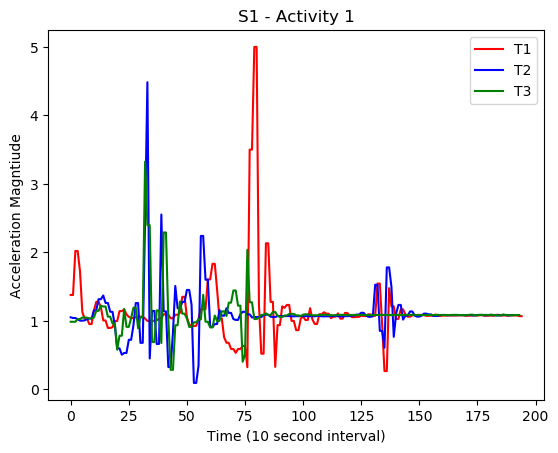
\includegraphics[width=5cm, height=4cm]{images/Acceleration/S1_Activity1.png} & 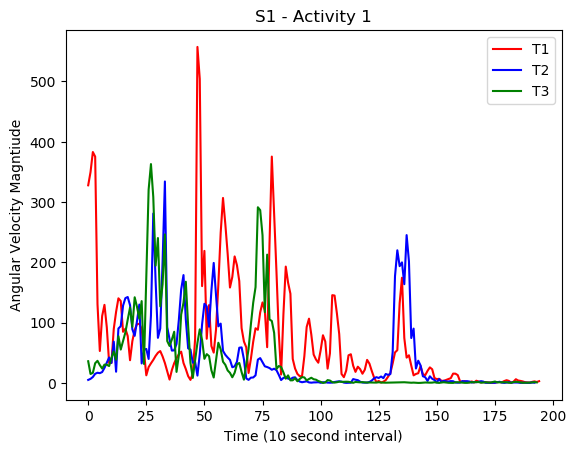
\includegraphics[width=5cm, height=4cm]{images/AngularVelocity/S1_Activity1.png}\\
			\midrule
			2 & 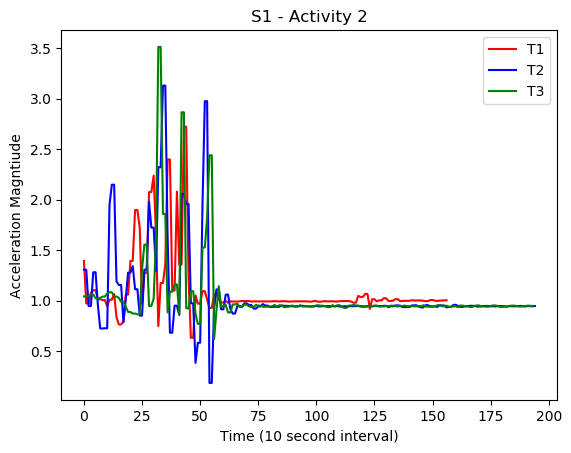
\includegraphics[width=5cm, height=4cm]{images/Acceleration/S1_Activity2.png} & 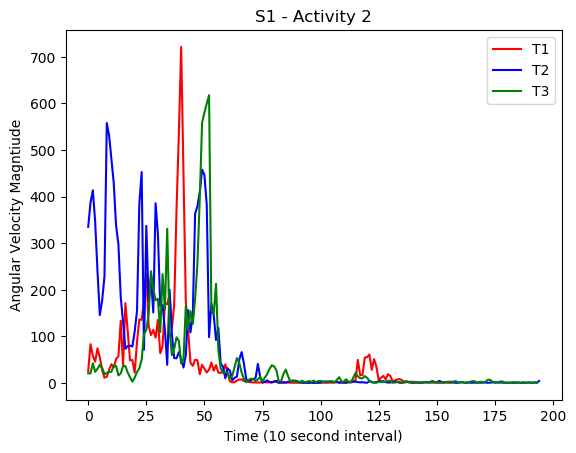
\includegraphics[width=5cm, height=4cm]{images/AngularVelocity/S1_Activity2.png}\\
			\midrule
			3 & 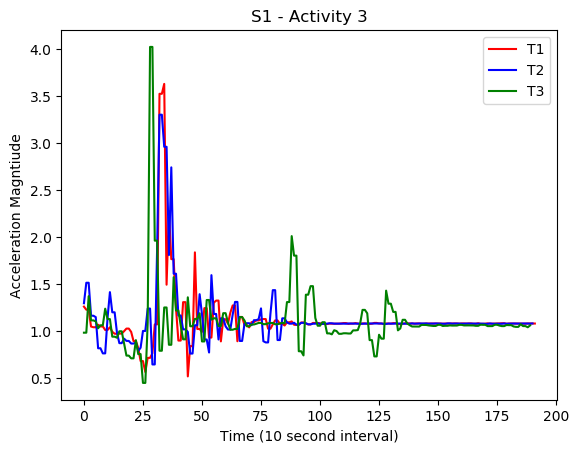
\includegraphics[width=5cm, height=4cm]{images/Acceleration/S1_Activity3.png} & 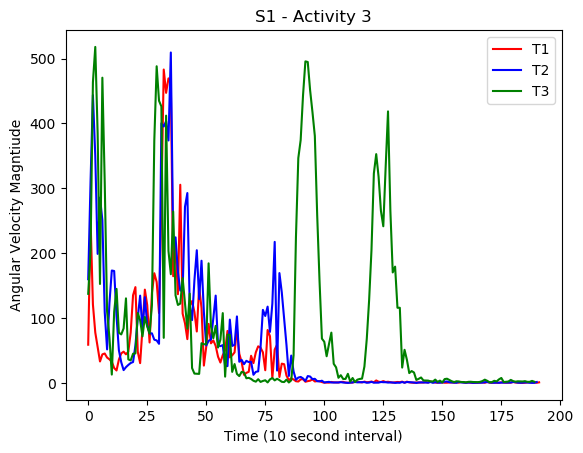
\includegraphics[width=5cm, height=4cm]{images/AngularVelocity/S1_Activity3.png}\\
			\midrule
			4 & 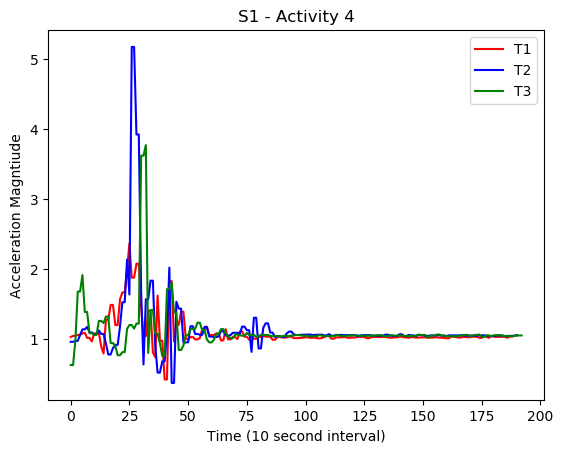
\includegraphics[width=5cm, height=4cm]{images/Acceleration/S1_Activity4.png} & 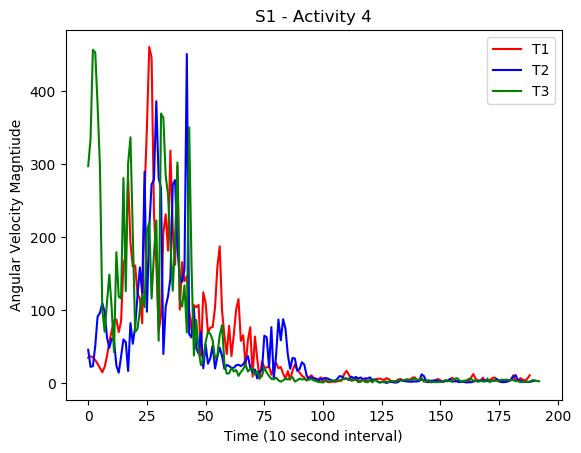
\includegraphics[width=5cm, height=4cm]{images/AngularVelocity/S1_Activity4.png}\\
			\midrule
			5 & 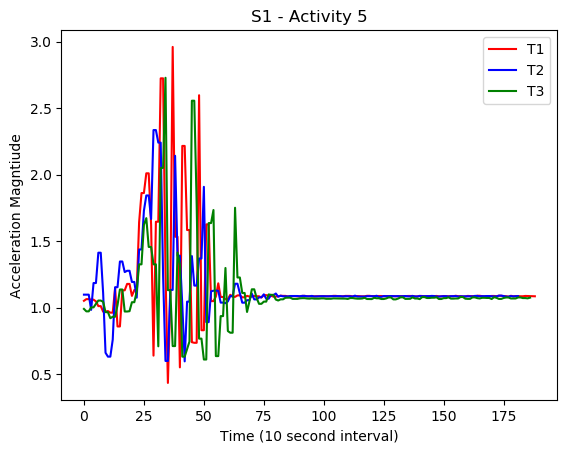
\includegraphics[width=5cm, height=4cm]{images/Acceleration/S1_Activity5.png} & 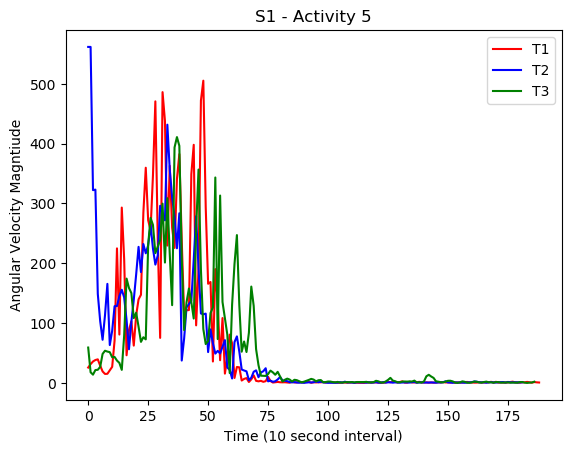
\includegraphics[width=5cm, height=4cm]{images/AngularVelocity/S1_Activity5.png}\\
			\bottomrule
		\end{tabular}
	\end{center}
\end{table}

The acceleration and angular velocity magnitude vector signals present as time series data of each simulated fall trial over the data collection interval. We use the peak value from these plot as potential threshold values to distinguish a fall from activities of daily living. However, the peaks occur at different maximum values for the five different types of simulated falls. The lower acceleration peaks for activities two and five with values of 3.0 and 3.5 appear to be a result of smaller distance displacements. The subject falls onto their knees from a standing position in activity 2 and falls from a seated position in activity five. In these two cases, the vertical displacement of the wrist sensor are smaller compared to the other falling simulations in which the subject falls from a standing position to the ground.

	We also define threshold values with vector changes of the acceleration and angular velocity magnitude signals. Instead of training the sensor to detect when a certain magnitude is measured, the model learns to detect motion intensity through magnitude changes. The Acceleration Vector Change (AVC) and Angular Velocity Vector Change (WVC) features are defined as:

	\begin{equation*}
    		AVC = \sum\limits_{i=1}^n \frac{| \vec{\mathbf{a}_{i}} - \vec{\mathbf{a}_{i-1}} |}{T_{n} - T_{0}}
	\end{equation*} 
	\begin{equation*}
		WVC = \sum\limits_{i=1}^n \frac{| \vec{\mathbf{w}_{i}} - \vec{\mathbf{w}_{i-1}} |}{T_{n} - T_{0}}
	\end{equation*} 

The absolute value of the summed differences between consecutive magnitude signals is divided by trial sampling period to produce the vector change value of a signal, where T\textsubscript{0} is the timestamp of the first data sample in a trial and T\textsubscript{n} is the last. When the sensors are not experiencing motion, the vector change for consecutive measurements will remain be constant. When motion is detected, the vector change value will measure the intensity of the motion with larger changes indicative of more forceful activity. 
	
	These processing steps resulted in 559 data instances that describe every trial executed by each of the 17 subjects for the 11 activities; two data points are missing because subject eight is missing sample signals for trials two and three in activity eleven. The raw triaxial sensor measurements, maximum magnitude values per trial, and signal vector changes were tested as candidate threshold values in our model. 
	
%by taking the maximum magnitudes for acceleration and angular velocity in each trial. The maximum value is the peak signal strength measured in a trial and represents a candidate threshold that must be attained to indicate that a certain activity is being performed.

% how was the data processed? PCA on raw triaxial measurements -> Maximum Magnitude Thresholds per Trial -> 
% investigate different feature extraction methods to 

\subsection{Methods}
%Detecting falls presents a myriad of technical, logistical, and practical challenges that we will need to address. From a modeling standpoint, an ADL-based dataset will have a very unbalanced response. This will also include a number of false flag activities, such as sitting or laying down. Additionally, falls can occur from multiple positions, such as standing, sitting, or many positions in between. This creates potential for both Type I and Type II error, and our model will need to be robust to both.
    
    %ADLs encompass a wide variety of activities, categorized into six different areas: bathing, ambulatory, transferring, toileting, eating, and dressing. These types of activity will inform our majority response and will be highly dominant in the data. Right away we can tell several of these pose a risk for falls, such as ambulatory or transferring. Transferring is defined as transitory periods from one activity to another, such as getting out of bed, sitting down to eat, getting in and out of chairs or vehicles, or going to sleep at night. Our model would need to know the difference between a transferal and a fall. This could be done by testing accelerometer data against the position in space, and check if the transition was the appropriate speed. 
    
    %This solution would not encompass all falls, and could ignore some important fall patterns. One common fall behavior, particularly in senior populations, is fainting during toileting. This can present an unexpected challenge - falls from a variety of different positions. If our model were only to expect falls to present a certain change in position at a certain rate, it would be unable to detect the aforementioned fall during toileting. The idea that not all falls are created equal will inform our model so that it can handle a variety of scenarios.
    
    %As mentioned before, this data will have a heavily unbalanced response, so appropriate measures will need to be taken to address this, such as downsampling and stratified cross validation. One possible method of addressing many of the previous challenges as well as dealing with the unbalanced response would be training the model for anomaly detection. This would require normalizing the variance across all ADLs, then treating that variance as the positive class of a binary response. The amount of data we have to train a positive response will be more than enough for an anomaly detection architecture.
    
   	% Methods - Paragraph 10 Defining the Fall
	%The first step is determining how we define a fall in the context of our algorithm. Fortunately, science defines this for us fairly succinctly in Newtonian physics, where any object upon which gravity is the only actor is said to be in free fall. A fall could be analyzed in much the same way - a person is said to be falling when gravity has more control of their movement than they or another person or device may have at that moment.
	
	%The question then becomes how we define a fall in the context of the algorithm. We already mentioned sensors and accelerometers as our tools of measuring a person's ADL and current state. Principle components or quadratic discriminants could be a simple method of measuring changes in state. Since we are not interested in the exact measurements in space - only types of changes - PCA or QDA could be a simple and efficient way of detecting changes. The challenge then becomes finding the range of the minority response.
	
	%Since there will be multiple types of falls, as well as falls that appear similar to other ADLs, establishing a threshold for falls - anomalies in this context - will be critical to this algorithm being successful. It is not reasonable to expect a small amount of anomalies to be sufficient in detecting any type of fall, nor all types. %Therefore, we plan to leverage methods such as reinforcement learning to solve this problem.
	% How will we define the threshold value for a fall?
		% picture a physics problem: *HP means hyper parameter*
			% an object in free fall [normalForce_up, gravitationalForce_down (HP: weight)]
			% an object at rest on the surface [dragForce_up (HP: dragCoefficient_up) , gravitationalForce_down (HP_constant: 9.8m/s^2]
	
	%At the crux of fall detection is striking a balance between exploiting the known (leaning on the knowledge of past falls) and exploring the unknown (discerning new falls and types of falls). Reinforcement learning is best suited to this task, as it will be key for this algorithm to seek to learn from past errors, both Type I and Type II, and reduce error going forward.
	
	%This has proven to be effective in past experiments with movement. Although there have been no uses in fall detection that we could find, researchers at the University of Porto have tested reinforcement learning in teaching robots to move in quicker, more efficient ways. By using a policy reuse algorithm, they were able to significantly improve the robot's gait when compared to other gait-improvement algorithms.\cite{garcia2020teaching}
	
	%Policy reuse could be particularly useful in our case. By maximizing the reward of our decision process, we can ensure our algorithm is more accurate with the more decision points we create. The challenge with this, again, is the unbalanced response. Without a handful of falls to train on, we still might not maximize this function. One way to counteract this is to introduce Monte Carlo methods. Even if our algorithm were to go into long periods of majority state, a Monte Carlo method would ensure continuous evaluation to make sure policies are improved.
	
	%All that said about falls, we need to give considerable thought to our majority response - ADLs. As described above, ADLs in their simplest form are motions of day-to-day life. While most movement scientists describe them in the six categories mentioned previously, there is some disagreement on that point. Many scientists do not feel that those six categories encompass the range of activities that should be included in the ADL category.
	
	%Researchers in Switzerland have proposed creating three very broad subcategories of ADLs based on their own fall detection research: basic movements, standard movements requiring some mobility, and sporting movements.\cite{casilari2017analysis} These ranges capture a broader population of ADLs and could serve us better in identifying our majority response. Additionally, since their work was based on more able-bodied adults, it would help us in crafting a more practically applicable model for wearable devices.
	
	%Speaking of practical significance, our choice to focus on wrist-based sensors was driven by a desire to match commonly preferred products on the market today, like Fitbit, Garmin, and Apple Watch. This choice brings its own set of benefits and challenges. Clear benefits include developing an algorithm that is more beneficial to a broader population. Most individuals concerned with falls will not want to wear sensors on their hips or heads, or multiple sensors, so a product that works only on the wrist will do the most good for the most people. 

	
	%Fortunately, methods have been developed to account for this accuracy issue with wrist-based sensors. Researchers tested four different hand-based ADLs - waving, knocking, clapping, and exercise - that frequently are mistaken for falls. Using ensemble stacked auto-encoders and one-class classification based on the convex hull (ESAEs-OCCCH), the researchers were able to generate a novel form of fall detection. This technique could be incorporated into our model to produce a more reliable metric from our sensors.\cite{chen2019method}

We compare the competing preprocessing methods by feeding the different features into our classification pipeline. K-means clustering identifies the acceleration and angular velocity threshold values that distinguish falls from other activities through centroid Euclidean distances. These distances are leveraged as class labels for falls and ADLs in a binary classification task using Support Vector Machines (SVM). 

\subsubsection{K-Means Clustering} 
Eleven clusters were initially tested to simulate the 11 different experimental activities, but these clusters did not provide clear separation between the different activities. Since specific values could not be identified for each activity, generalized threshold values for falls and ADLs were identified using two cluster centroids in the k-means clustering algorithm. Figure one presents the results of the clustering analysis with two identified centroids displaying separation between the simulated falls and ADLs. Since the sensor experiences more force during the event of a fall, the k-means centroid for falls (red data points) has larger threshold values for acceleration and angular velocity compared to ADLs (green data points) as expected. The vector change threshold values from the fall cluster are 6.891 g for acceleration and 897.310 deg/s for angular velocity. The vector change threshold values from the ADL cluster are 0.955 g for acceleration and 241.720 deg/s for angular velocity. 

\begin{figure}
	\centering
	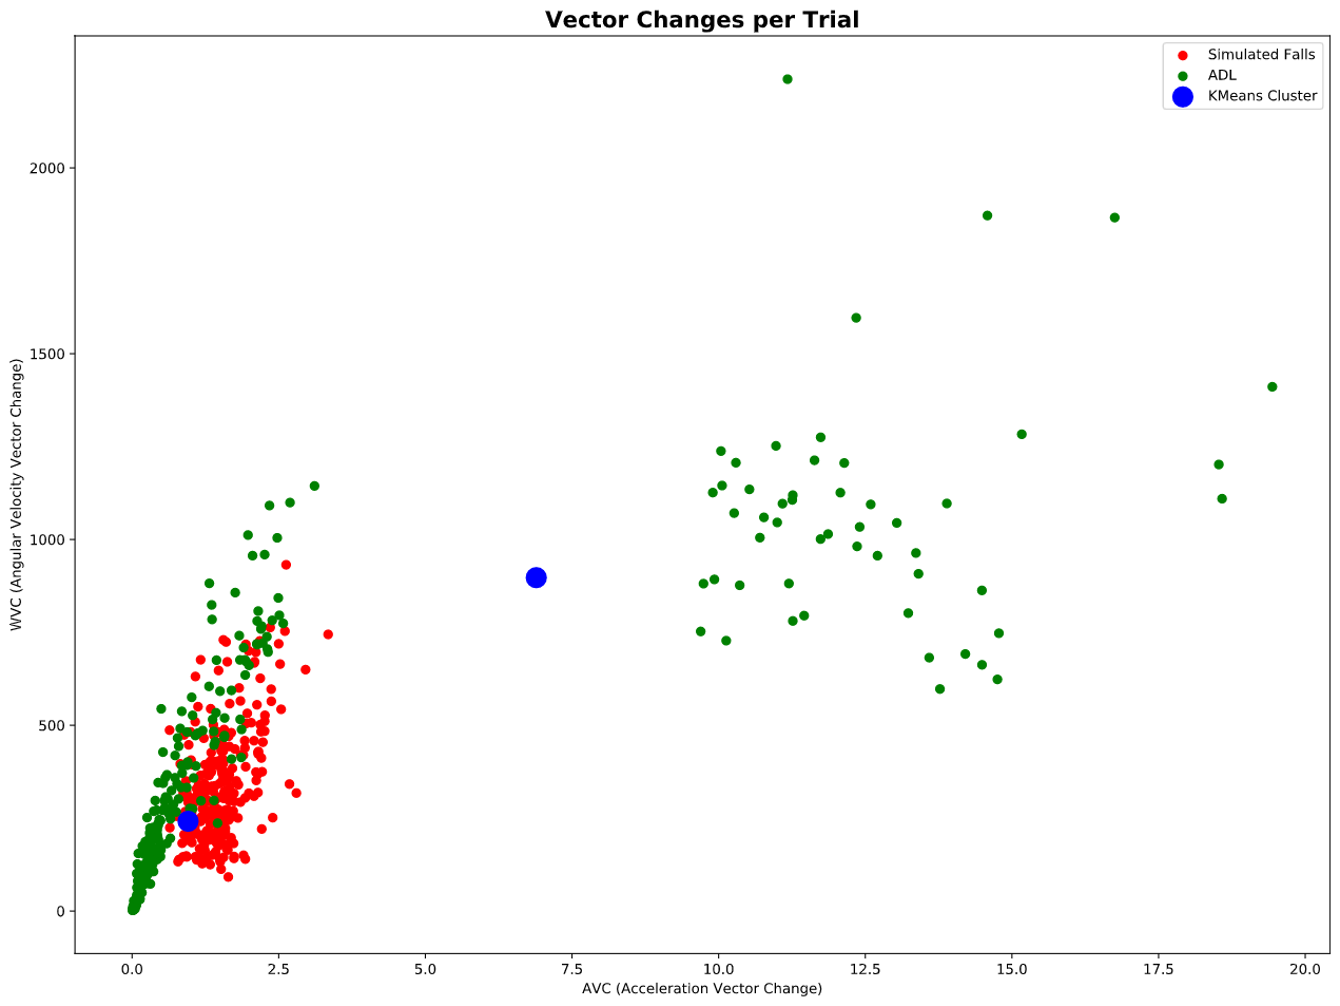
\includegraphics[width=12cm, height=10cm]{images/VC_2clusters.png} 
	\caption{: K-Means Fall and ADL Class Centroids for AVC \& WVC thresholds}
	\label{Figure 1: 2 Clusters}
\end{figure}
% K-Means Centroids of Falls and ADLs on Max Acceleration and Angular Velocity Magnitudes

	In addition to acceleration and angular velocity changes, the threshold analysis also tests raw sensor measurements on individual axes and maximum magnitude signals as well. Principal Components Analysis (PCA) is used to reduce the triaxial measurements to a smaller feature set representing the signals measured by the accelerometer and gyroscope in each trial. Alternatively, maximum magnitude signals from each trial were extracted as another processing technique to reduce data dimensionality and represent potential thresholds for each of the two sensors. Table four summarizes the centroid distance extracted from k-means clustering for each of the competing threshold types. These centroid distances represent threshold values that are used as input labels for distinguishing falls from activities of daily living in a SVM classifier. 
	
%\begin{table}
%	\begin{center}
%		\caption{Maximum Triaxial Threshold Measurements}
%		\label{table4}
%		\begin{tabular}{|c|c|c|}
%			\toprule
%			Axis & Acceleration Threshold (g) & Angular Velocity Threshold (deg/s)\\
%			\midrule
%			X & \makecell{1.424 (Fall)\\0.859 (ADL)} & \makecell{487.244 (Fall)\\181.375 (ADL)}\\
%			Y & \makecell{1.359 (Fall)\\0.621 (ADL)} & \makecell{289.069 (Fall)\\135.140 (ADL)}\\
%			Z & \makecell{1.589 (Fall)\\1.136 (ADL)} & \makecell{314.613 (Fall)\\126.999 (ADL)}\\
%			\bottomrule
%		\end{tabular}
%	\end{center}
%\end{table}
	
 \begin{table}
 	\begin{center}
		\caption{Summary of Magnitude Threshold Values to be Tested in Classifier}
		\label{table4}
		\begin{tabular}{|c|c|c|}
			\toprule
			Threshold Type & Acceleration Threshold (g) & Angular Velocity Threshold (deg/s)\\
			\midrule
			Triaxial Measurements (PCA) & \makecell{2.530 (Fall) \\1.554 (ADL)} & \makecell{648.035 (Fall) \\259.401 (ADL)}\\
			\midrule
			Maximum Magnitude & \makecell{3.502 (Fall) \\2.331 (ADL)} & \makecell{694.076 (Fall) \\292.689 (ADL)}\\
			\midrule
			AVC \& WVC & \makecell{6.891 (Fall) \\0.955 (ADL)} & \makecell{897.310 (Fall) \\241.720 (ADL)}\\
			\bottomrule
		\end{tabular}
 	\end{center}
\end{table} 

\subsubsection{Support Vector Machine Classification} 
Support Vector Machines is a supervised machine learning technique that projects labeled training data onto a higher dimensional space. A decision boundary is then defined to linearly separate categorical class labels by maximizing its orthogonal distances from support vectors. In two dimensions the decision boundary can be defined as a line, but in n-dimensions it is best defined as a hyperplane with (n-1)-dimensions. Support vectors are the data instances closest to the defined closest to the boundary line on each side of the class labels. 

	With non-linearly separable data, transformation kernel tricks are employed to map the data into a different dimensionality space so that the SVM algorithm can better identify a hyperplane capable of linearly separating classes. A variety of kernels (i.e., linear, sigmoid, polynomial, Gaussian) are tested on the k-means feature space to evaluate the best parameters for the binary classification of falls from activities of daily living. Accuracy, recall, precision, and F\textsubscript{1} score are used as comparative metrics to quantify the performance of competing models. In order to leverage the k-means labeling of fall and ADL threshold values, the centroid distance vectors from the different data processing methods were fed into a Support Vector Classifier (SVC) as input criteria.

%	We use a SVM to classify centroid distances generated from k-means to predict falls vs ADLs. We will need to test a variety of kernels, since the k-means feature space may or may not be linear, quadratic, or possibly separable in a 3D feature space. Accuracy and precision are used as comparative metrics to quantify how competing models .

%  Since we used similar clustering methods for both the triaxial and magnitude models, we tested SVC models of linear, polynomial, sigmoid,  kernels on each cluster method, for a total of six classification tests. 
    
\section{Results}

The raw triaxial measurements provided two distance vectors per axis for a total of six vectors. PCA was applied to the six feature vectors to reduce the data dimensionality of the binary classification task to two components. These principal component values were then used to compute 2 k-means centroid distances for fall and ADL class labels in an SVM classifier tested with different kernels. The results are represented in the 3D scatterplot shown in Figure two.

%To reduce dimensionality in the classification, we applied Principle Component Analysis with two components, representing each sensor signal in order to reduce the dimensionality required for classification.
%\begin{table}
% 	\begin{center}
%		\caption{SVM Classifier Accuracy for Triaxial Distance Components By Kernel}
%		\label{table5}
%		\begin{tabular}{|c|c|}
%			\toprule
%			Kernel Type & Accuracy Percent\\
%			\midrule
%			Linear Kernel & \makecell{52.972}\\
%			Polynomial Kernel & \makecell{52.972}\\
%			Gaussian Kernel & \makecell{50.622}\\
%			\bottomrule
%		\end{tabular}
 %	\end{center}
%\end{table} 
    
\begin{figure}
	\centering
	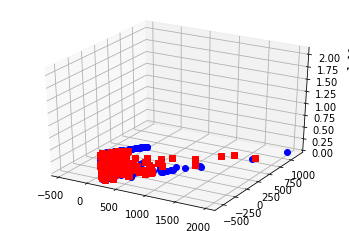
\includegraphics[width=12cm, height=10cm]{images/Classification/3D_PCA.png} 
	\caption{: 3D PCA Decision Boundary of Triaxial Distance Components}
	\label{Figure 2: 3D Plot of Linear Kernel SVM with Triaxial Distance Components}
\end{figure}    

Many of the predictions are clustered around a single point in space and are not easily separated linearly by projecting to a higher dimensional plane. This is reflected in the low accuracy around 50 percent regardless of the kernel selected for SVM classification. Given this low performance and lack of response to parameter tuning, maximum magnitude signals from each trial were instead used as a processing step to extract threshold values for classification.
	
	Linear, sigmoid, polynomial, and Gaussian kernels were again tested on the maximum magnitude signals. These values provided higher accuracy than the PCA components of raw triaxial sensor measurements with the linear kernel yielding the most significant performance in comparison to the other kernels at 67\%. The linear kernel yielded the most significant performance improvement in comparison to the other kernels and the raw triaxial sensor measurements. Figure three shows the hyperplane decision boundary from the SVM classifier on maximum magnitude signal thresholds using a linear kernel.
	
\begin{figure}
	\centering
	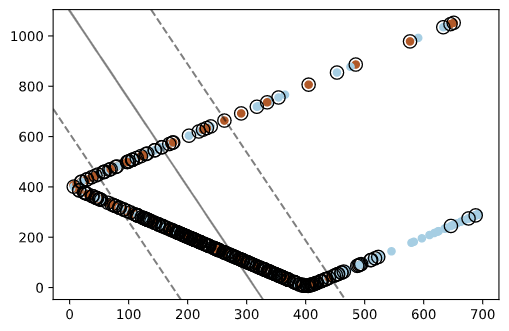
\includegraphics[width=12cm, height=10cm]{images/Classification/linear_classifier_boundary.png} 
	\caption{: Linear SVM Classifier of Maximum Magnitude Thresholds}
	\label{Figure 3: Linear Kernel SVM with Magnitude Thresholds Hyperplane}
\end{figure} 	

Many of the data points appear to be clustered in an elbow shape around the origin, with most representing the majority class. This likely accounts for the improvement in accuracy, but does not significantly increase the precision. To account for some of these issues, we shifted our threshold analysis to vector change features from the accelerometer and gyroscope sensors to better measure motion intensity. Acceleration Vector Change (AVC) and Angular Velocity Vector Change (WVC) values per trial were pushed through the classification pipeline to identify class labels through k-means and predict fall instances from ADLs in a binary SVM classifier.
	
	%Similar to the triaxial model, the magnitude cluster model provided two distance vectors, but since we had created one cluster model using both magnitude thresholds, there was no need for dimensionality reduction. Therefore, the distance vectors were passed to the SVM classifier in their raw form. Again, we repeated these tests on linear, polynomial, and sigmoid kernels. We observed significant improvement in using a linear kernel on these distances. Although still not very accurate, a roughly 67 percent accuracy performs much better than the other kernels and the triaxial component model. A plot of the decision boundary is below.
    
%\begin{table}
 %	\begin{center}
%		\caption{SVM Classifier Accuracy for Magnitude Distance By Kernel}
%		\label{table5}
%		\begin{tabular}{|c|c|}
%			\toprule
%			Kernel Type & Accuracy Percent\\
%			\midrule
%			Linear Kernel & \makecell{67.000}\\
%			Polynomial Kernel & \makecell{51.891}\\
%			Gaussian Kernel & \makecell{58.900}\\
%			\bottomrule
%		\end{tabular}
 %	\end{center}
%\end{table} 
		
	Figure four shows that the k-means centroid classification task using vector change features produces a much narrower hyperplane, along with the same elbow shape seen in the previous classifier. The vectors are much more closely clustered around the hyperplane as well. Unlike the previous classifier, the linear separation is more clear between the ADL vectors and the fall vectors. This will yield higher accuracy, and more importantly, higher precision on the classification task. The outliers are still present but are on the correct side of the decision boundary. One concern with the narrowness of the hyperplane is the possibility of misclassification in the case of vectors that are slightly further away from the support vectors. We will want to examine recall to ensure this is not a potential weakness.
	
\begin{figure}
	\centering
	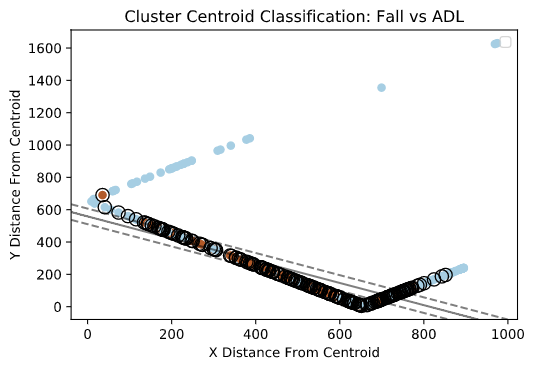
\includegraphics[width=12cm, height=10cm]{images/Classification/linear_classifier_boundary_avc.png} 
	\caption{: Linear SVM Classifier of AVC and WVC}
	\label{Figure 4: Linear Kernel SVM with AVC and WVC Hyperplane}
\end{figure}
        

% Put in discussion when talking about outliers - show activity labeled K-means plot and talk about jumping -> 
    %There are a significant grouping of ADL outliers. For the time-being, we will ignore these and proceed with classification. Since we have had the greatest success with the SVM linear kernel, we will classify the centroid distances of the AVC model with this classifier as well.

	Despite the presence of outliers, this vector change model performed the best with an overall accuracy of 78.4\%. The linear decision plot appears similar to the magnitude model, but predict ADL labels further away from the decision boundary. This aligns with what is seen in the cluster plot, and could explain the increase in accuracy from the previous model. A final comparison of the performance metrics from our top-competing models is shown in table five.
    
\begin{table}
 	\begin{center}
		\caption{SVM Classifier Accuracy for AVC Distance By Kernel}
		\label{table5}
		\begin{tabular}{|c|c|c|c|c|c|}
			\toprule
			Pre-Processing & Kernel Type & Accuracy & Precision & Recall & F\textsubscript{1} Score\\
			\midrule
			AVC & Linear Kernel & \makecell{78.400\%} & \makecell{74.200\%} & \makecell{82.800\%} & \makecell{78.300\%}\\
			Magnitude Threshold & Linear Kernel & \makecell{67.000\%} & \makecell{63.800\%} & \makecell{69.00\%} & \makecell{66.300\%}\\
			Magnitude Threshold & Gaussian Kernel & \makecell{58.900\%} & \makecell{58.500\%} & \makecell{43.700\%} & \makecell{50.000\%}\\
			\bottomrule
		\end{tabular}
 	\end{center}
\end{table}     

	The linear kernel SVM classification on k-means centroid distances of vector change features showed significant improvement across all metrics from previous models. This model appears to address some of the precision issues in current fall detection algorithms on solely wrist sensor data with a competitive measure of 74.2\% indicating low false positive rates. Precision weighs the costs of false positive predictions (i.e., predicting an activity of daily living to be a fall). Recall weighs the costs of false negative predictions (i.e., predicting a fall to be an activity of daily living). At 82.8\% recall, our model performs even better in regards to actually identifying relevant instances as falls and not mislabelling them as an ADL. The F\textsubscript{1} score metric is the harmonic mean of precision and recall, meaning it weighs model performance with false positive and false negative costs over true negative predictions. The F\textsubscript{1} Score of 78.3\% is comparable to the overall classification accuracy of 78.4\%, indicating a balanced model that is accurate, precise, and generalizable. 

\section{Discussion}
% add quick summary of methodology from figure 5

\begin{figure}
	\centering
	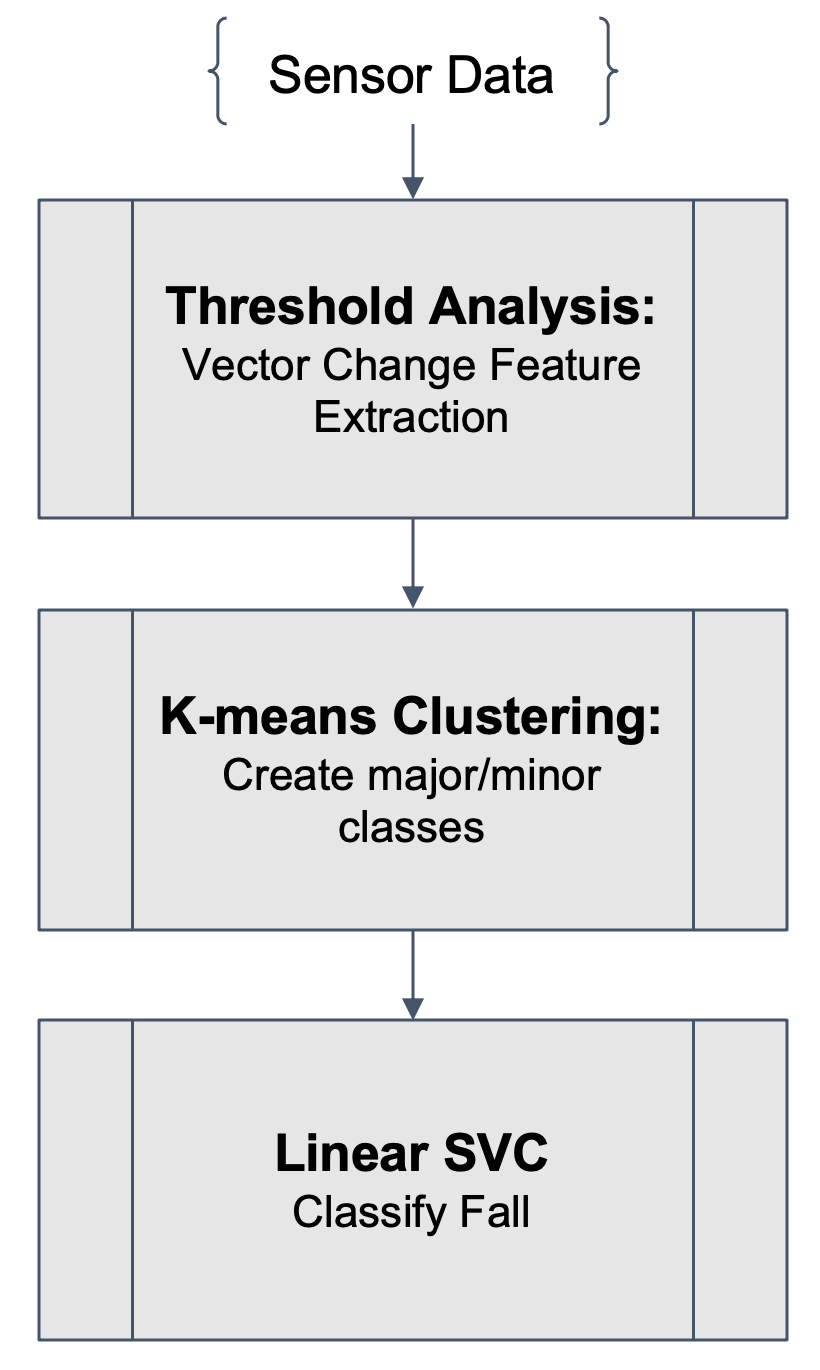
\includegraphics[width=5cm, height=8cm]{images/ClassificationPipeline.png} 
	\caption{: 3-Phased Model Approach}
	\label{Figure 5: Threshold Analysis Classification Pipeline}
\end{figure}
%@Michael cite this paragraph with link: just place link in url bracket and uncomment
As mentioned in the results, our final 3-phased threshold analysis model approach (AVC to K-Means to SVM) had an accuracy of about 78 percent. Although there is sparse research on the efficacy of existing fall detection systems outside laboratory settings, owing to manufacturers being reticent to releasing that information, many consumer studies report similar accuracy to our result. However, unlike these products our model is much more precise, at 74 percent.%\footnote{\url{}} 

	As mentioned in the results, our final model (AVC to K-Means to SVM) had an accuracy of about 78 percent. Although there is sparse research on the efficacy of existing fall detection systems outside laboratory settings, owing to manufacturers being reticent to releasing that information, many consumer studies report similar accuracy to our result.\cite{medreview} However, unlike these products our model is much more precise, at 74 percent. 
	
	A potential concern was noted when plotting the decision boundary - the possibility of misclassification due to narrowness in the hyperplane. Although the data on which we trained the model produced a good recall score (over 82\%) it is worth exploring some possible strategies to make the model more adaptable and resilient. Outliers were observed in the formed AVC and WVC k-means centroid clusters. These data points with larger vector change values for acceleration and angular velocity were identified to be from trials of activity ten as shown in figure five. Activity ten from the data iss jumping, which consists of continuous acceleration changes over the trial period. Given the nature in which vector changes were calculated over the entire trial period, a jumping activity would generate large a vector change value due to continuous motion over a 30 second window and manifest as outliers in the data.

	In order to address this issue, an optimal window for vector change thresholds needs to be defined so that motion intensity can be better measured in small time frames. In this way, threshold values can better capture large, sudden changes in acceleration and angular velocity vectors that are more characteristic of fall events. This is an important distinction as the stimulated falls (activities one through five) are sampled in 10 second trial periods compared to the the majority of stimulated ADLs (activities six through eleven) are mostly sampled in 30 or 60 second trial periods. An optimal sampling window for vector change thresholds would improve signal processing by ensuring that sudden, large vector changes measured by the sensor can be attributed to intense motions rather than continuous motion.
	
	Prior research investigated the use of Butterworth filters to remove noise such as gravitational acceleration from the raw triaxial sensor signals as an effective signal processing technique.\cite{hussainelderly2019} With noise effectively filtered from these signals, an acceleration component characteristic of just the detected motion can be isolated and provide vector change thresholds that are more representative of pure human motion. 

\begin{figure} 
	\centering
	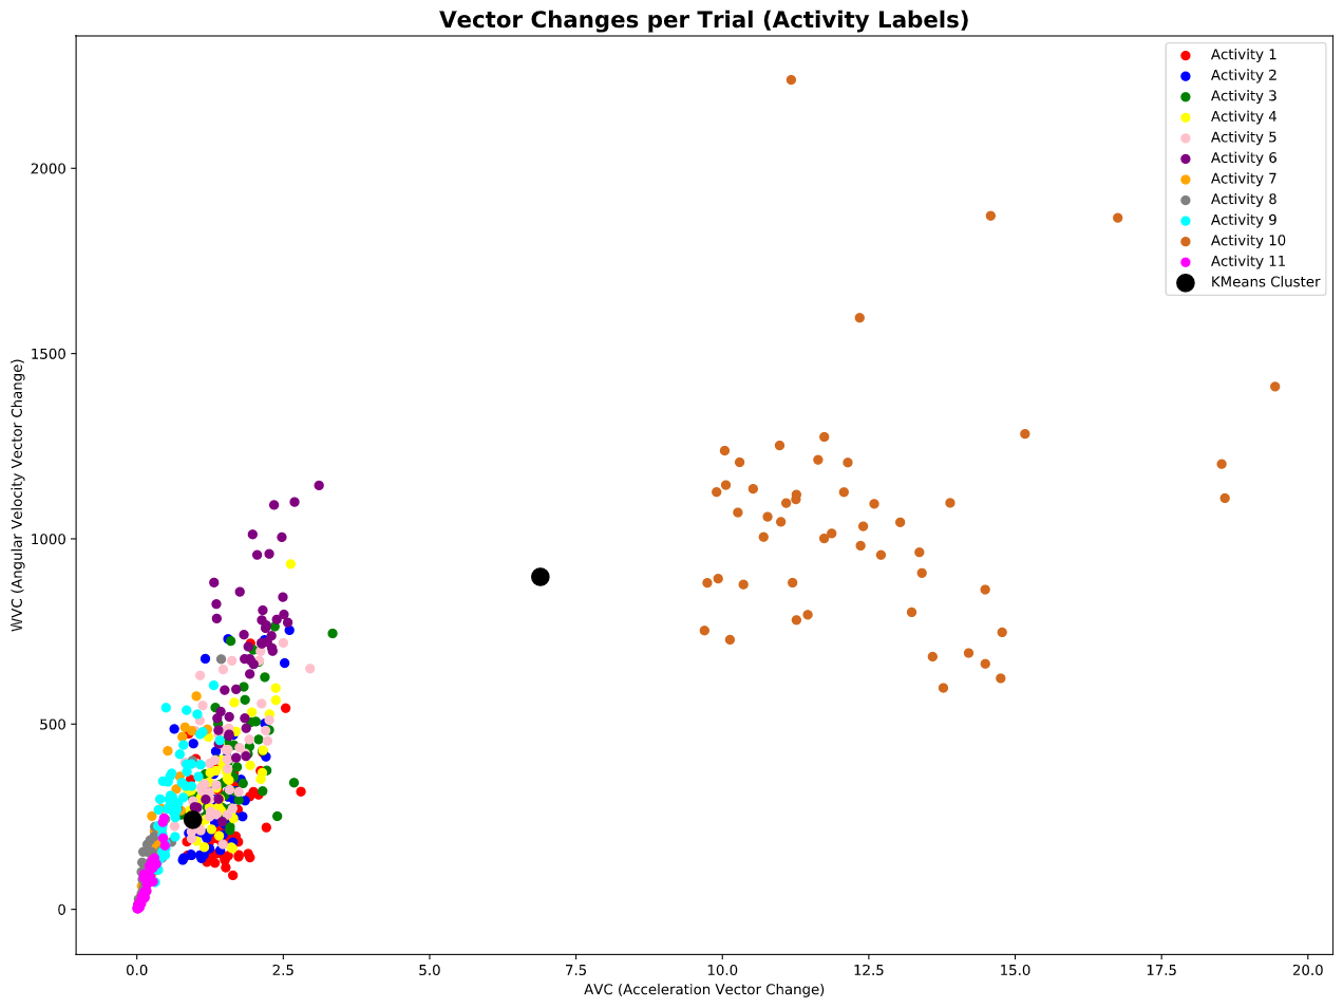
\includegraphics[width=12cm, height=10cm]{images/VC_11clusters.png} 
	\caption{: AVC \& WVC highlighted by activity}
	\label{Figure 6: K-Means Clusters of AVC and WVC Values per Trial}
\end{figure}
	
	A knowledge-based multiphase fall model approach has been researched to address many of the technical challenges of an autonomous fall detection system and yielded overall performances of 99.79\% sensitivity, 98.74\% specificity, 99.05\% precision, and 99.33\% accuracy.\cite{hsieh2017novel} The multiphase approach introduces free fall, impact and rest phases to characterize a fall. These three phases characterize a window of a drastic increase in acceleration, succeeded by a rapid decrease in acceleration, and ends with an extended period of constant acceleration. In the free-fall phase, the acceleration vector change signal should mimic gravitational acceleration and could be extracted using Butterworth filters as previously discussed. The impact phase can be characterized as a large, negative vector change within a small time window. The rest phase should be attributed with a vector change value of 0 over a few seconds. Applying vector change features and machine learning based approaches to this multiphase model potentially offers a potentially viable solution to an autonomous fall detection system developed from threshold analysis of wrist sensor data.

	As a real-world application, our model can be integrated into modern-day wearable technologies such as smartwatches to leverage their built-in Global Positioning System (GPS). In the event a fall results in incapacitation, the autonomous fall detection system can dispatch emergency medical services to the pinpoint location of the device. The imprecision of existing systems is a barrier for such a development, and we believe introducing a more precise model such as ours will ensure broader adoption by rectifying this issue.

% Add AVC to multiphase-fall model: free fall, impact, rest phases

% Add high-pass, low-pass, or Butterworth band filter to remove gravity etc.

% Optimize AVC window to capture sudden changes 

	%Similar to previous pre-processing methods, we still see significant outliers, categorically on Activity Ten (jumping). Given that this new pre-processing step would produce larger vector changes for activities that involve sudden acceleration changes, this is expected. We will proceed with classification.


\subsection{Ethics}

One major ethical consideration, both within this analysis and others on fall detection, is bias within the data. Pre-existing publicly available datasets often contain data sourced from healthy adults who predominantly skew younger and male.\cite{casilari2017analysis} Studies that generate their own data frequently recruit people of similar demographics because of the health and safety concerns posed by attempting to source data from the elderly.\cite{gjoreski2016accurately} Any data that is generated by older adults is often limited to ADLs as opposed to falls. Although volunteers are often coached to simulate fall behavior in a similar fashion to the elderly, factors like predefined movements, test environments that do not well approximate where the elderly are most likely to fall, and the presence of safety precautions like mattresses could all result in simulated fall data that does not actually match the reality.\cite{casilari2017analysis} Kangas et al. demonstrate that the profiles for a small number of real-life falls look similar to those of simulated ones.\cite{kangas2008comparison} However, we caution against assuming this extends to other simulated data and recommend more investigation into the possible influence of demographic bias and safety measures.
	
	Another potential ethical consideration is privacy. In a similar fashion to how personalized medicine tailors to individual patients, a user-centric model that trains on the wearer's baseline ADL movements has been suggested to perform better than a generalized one.\cite{villar2019online} Manufacturers of wrist wearables could allow users to opt-in to providing their real-life ADL data to refine the generalized model that the user-centric model works with. However, this introduces realistic concerns over whether user information is properly removed or anonymized in the event of data breaches.

   % Minimal invasiveness of wrist sensor placement compared to head, torso, or waist.
    
%\section{Discussion}
\section{Conclusion}

Our study uses a subset of the UP-Fall Detection dataset to analyze acceleration and angular velocity signals measured on wrist-worn sensors to simulate smartwatch placement. We designed a threshold-based model on a binary classification task to distinguish falls from activities of daily living. We found that vector change features capturing the collective sum of differences between consecutive signals in time provided the most accurate model. The Acceleration Vector Change (AVC) and Angular Velocity Vector Change (WVC) features were inputted into a K-Means Clustering algorithm to identify two k-means centroids: one for falls and one for activities of daily living (ADL). The centroid distances represent the threshold values that AVCs and WVCs must reach to classify a fall. The two centroids with AVC and WVC distances were fed into a Support Vector Machine (SVM) classifier with a linear kernel and yielded an accuracy of 78.4\%. 

	Due to the use of the trial period as the processing time window for vector change features, activities consisting of continuous motions created outliers in the data. Activity 10, jumping, from the dataset was the example previous discussed. Thus, the processing time window should be lowered to an optimal period that better capture sudden, large changes in the acceleration and angular velocity magnitude vectors. Smaller time windows will provide a better representation of vector changes for individual motions rather than continuous. 
	
	Previous research on fall detection systems lend insight into techniques that can further refine our proposed model. Signal processing techniques such as Butterworth filters have been used to remove background noise from the triaxial accelerometer and angular velocity sensors to extract a signal that is more characteristic of pure human motion. A knowledge-based multiphase model characterizing distinct free fall, impact, and rest states for fall detection systems has provided extremely accurate results across performance metrics. 

	The objective of our proposed solution for novel autonomous fall detection systems is to provide a model that can be applied to wrist-wearable technologies with accelerometer and gyroscope sensors. We must caution extrapolating this model to the senior population as it was only trained on a sample population of young, healthy adults aged 18-24 years old. Many current commercialized smartwatch devices also have built-in GPS that our application can further take advantage of by dispatching local paramedics to an exact location if a fall is detected in order to minimize the dangers of a ``long-lie'' condition.

%The overall accuracy of the SVM classifier was low, until the AVC pre-processing step was added. The final, most accurate classifier was a linear kernel on AVC cluster, at 78.4\% percent. As mentioned above, there are many points clustered near the origin, suggesting a high rate of true negatives contributing to the overall accuracy. Additionally, another possible method could be Gaussian mixture model, which would essentially create both components (labelling plus classification) in a single process, although we would need to indicate or compute a threshold of probability for this to work practically.

	%The high number of outliers in the cluster analysis is also worth mentioning. Interestingly, most of these outliers corresponded with Activity ten, or the jumping activity. Although removing this does not improve accuracy by much, it does present an interesting observation: clusters of AVCs are more linearly separable for fall-like acceleration versus other activities.  

	%To further our analysis and the performance of our fall detection algorithm, better signal processing techniques should be employed to represent the time series data in each trial. In this analysis, taking the maximum values of the magnitude of the sensor signal caused all other measurements in each trial besides the peak signal to be discarded. Combinations of high-pass filters on the time series and regression analysis to extract a singular representative value for each trial are recommended as improvements over the current signal processing technique of taking the maximum value. 

	%We propose a novel autonomous fall-detection system using algorithms trained on data extracted from wireless accelerometer and gyroscope wrist sensors as a potential solution to address these concerns. When our algorithm detects a fall and the user is unable to confirm consciousness through the wrist device, it could trigger an alert to dispatch local paramedics to the device's exact GPS location for an emergency evaluation and immediate medical intervention. %The algorithm is tasked with a binary classification that will discriminate actual falls from typical activities of daily living: bathing, ambulatory, transferring, toileting, eating, and dressing.




% ---- Bibliography ----
%
% BibTeX users should specify bibliography style 'splncs04'.
% References will then be sorted according to alphabetical 
% and formatted in the correct style.
%


 \bibliography{Fall+Detection_Final}{}
 \bibliographystyle{splncs04}

% End the Document
\end{document}